%%%%%%%%%%%%%%%%%%%%%%%%%%%%%%%%%%%%%%%%%
% Article EcoFoG
% Version 2.1 (23/10/2017)
%
% adapté de :
% Stylish Article
% LaTeX Template
% Version 1.0 (31/1/13)
%
% This template has been downloaded from:
% http://www.LaTeXTemplates.com
%
% Original author:
% Mathias Legrand (legrand.mathias@gmail.com)
%
% License:
% CC BY-NC-SA 3.0 (http://creativecommons.org/licenses/by-nc-sa/3.0/)
%
%%%%%%%%%%%%%%%%%%%%%%%%%%%%%%%%%%%%%%%%%


%----------------------------------------------------------------------------------------
%	PACKAGES AND OTHER DOCUMENT CONFIGURATIONS
%----------------------------------------------------------------------------------------

\documentclass[fleqn,10pt]{ArtEcoFoG} % Document font size and equations flushed left

\setcounter{tocdepth}{3} % Show only three levels in the table of contents section: sections, subsections and subsubsections


% Pandoc environments
\usepackage{framed}
\usepackage{fancyvrb}
\providecommand{\tightlist}{%
  \setlength{\itemsep}{0pt}\setlength{\parskip}{0pt}}
\newcommand{\VerbBar}{|}
\newcommand{\VERB}{\Verb[commandchars=\\\{\}]}
\DefineVerbatimEnvironment{Highlighting}{Verbatim}{commandchars=\\\{\}, fontsize=\scriptsize} % Code R
\definecolor{shadecolor}{RGB}{248,248,248}
\newenvironment{Shaded}{\begin{snugshade}}{\end{snugshade}}
\newcommand{\KeywordTok}[1]{\textcolor[rgb]{0.13,0.29,0.53}{\textbf{{#1}}}}
\newcommand{\DataTypeTok}[1]{\textcolor[rgb]{0.13,0.29,0.53}{{#1}}}
\newcommand{\DecValTok}[1]{\textcolor[rgb]{0.00,0.00,0.81}{{#1}}}
\newcommand{\BaseNTok}[1]{\textcolor[rgb]{0.00,0.00,0.81}{{#1}}}
\newcommand{\FloatTok}[1]{\textcolor[rgb]{0.00,0.00,0.81}{{#1}}}
\newcommand{\ConstantTok}[1]{\textcolor[rgb]{0.00,0.00,0.00}{{#1}}}
\newcommand{\CharTok}[1]{\textcolor[rgb]{0.31,0.60,0.02}{{#1}}}
\newcommand{\SpecialCharTok}[1]{\textcolor[rgb]{0.00,0.00,0.00}{{#1}}}
\newcommand{\StringTok}[1]{\textcolor[rgb]{0.31,0.60,0.02}{{#1}}}
\newcommand{\VerbatimStringTok}[1]{\textcolor[rgb]{0.31,0.60,0.02}{{#1}}}
\newcommand{\SpecialStringTok}[1]{\textcolor[rgb]{0.31,0.60,0.02}{{#1}}}
\newcommand{\ImportTok}[1]{{#1}}
\newcommand{\CommentTok}[1]{\textcolor[rgb]{0.56,0.35,0.01}{\textit{{#1}}}}
\newcommand{\DocumentationTok}[1]{\textcolor[rgb]{0.56,0.35,0.01}{\textbf{\textit{{#1}}}}}
\newcommand{\AnnotationTok}[1]{\textcolor[rgb]{0.56,0.35,0.01}{\textbf{\textit{{#1}}}}}
\newcommand{\CommentVarTok}[1]{\textcolor[rgb]{0.56,0.35,0.01}{\textbf{\textit{{#1}}}}}
\newcommand{\OtherTok}[1]{\textcolor[rgb]{0.56,0.35,0.01}{{#1}}}
\newcommand{\FunctionTok}[1]{\textcolor[rgb]{0.00,0.00,0.00}{{#1}}}
\newcommand{\VariableTok}[1]{\textcolor[rgb]{0.00,0.00,0.00}{{#1}}}
\newcommand{\ControlFlowTok}[1]{\textcolor[rgb]{0.13,0.29,0.53}{\textbf{{#1}}}}
\newcommand{\OperatorTok}[1]{\textcolor[rgb]{0.81,0.36,0.00}{\textbf{{#1}}}}
\newcommand{\BuiltInTok}[1]{{#1}}
\newcommand{\ExtensionTok}[1]{{#1}}
\newcommand{\PreprocessorTok}[1]{\textcolor[rgb]{0.56,0.35,0.01}{\textit{{#1}}}}
\newcommand{\AttributeTok}[1]{\textcolor[rgb]{0.77,0.63,0.00}{{#1}}}
\newcommand{\RegionMarkerTok}[1]{{#1}}
\newcommand{\InformationTok}[1]{\textcolor[rgb]{0.56,0.35,0.01}{\textbf{\textit{{#1}}}}}
\newcommand{\WarningTok}[1]{\textcolor[rgb]{0.56,0.35,0.01}{\textbf{\textit{{#1}}}}}
\newcommand{\AlertTok}[1]{\textcolor[rgb]{0.94,0.16,0.16}{{#1}}}
\newcommand{\ErrorTok}[1]{\textcolor[rgb]{0.64,0.00,0.00}{\textbf{{#1}}}}
\newcommand{\NormalTok}[1]{{#1}}
\usepackage{longtable,booktabs}
\usepackage{caption}
% These lines are needed to make table captions work with longtable:
\makeatletter
\def\fnum@table{\tablename~\thetable}
\makeatother
% longtable 2 columns
% https://tex.stackexchange.com/questions/161431/how-to-solve-longtable-is-not-in-1-column-mode-error
\makeatletter
\let\oldlt\longtable
\let\endoldlt\endlongtable
\def\longtable{\@ifnextchar[\longtable@i \longtable@ii}
\def\longtable@i[#1]{\begin{figure}[t]
\onecolumn
\begin{minipage}{0.5\textwidth}\scriptsize
\oldlt[#1]
}
\def\longtable@ii{\begin{figure}[t]
\onecolumn
\begin{minipage}{0.5\textwidth}\scriptsize
\oldlt
}
\def\endlongtable{\endoldlt
\end{minipage}
\twocolumn
\end{figure}}
\makeatother

\usepackage{graphicx,grffile}
\makeatletter
\def\maxwidth{\ifdim\Gin@nat@width>\linewidth\linewidth\else\Gin@nat@width\fi}
\def\maxheight{\ifdim\Gin@nat@height>\textheight0.8\textheight\else\Gin@nat@height\fi}
\makeatother
% Scale images if necessary, so that they will not overflow the page
% margins by default, and it is still possible to overwrite the defaults
% using explicit options in \includegraphics[width, height, ...]{}
\setkeys{Gin}{width=\maxwidth,height=\maxheight,keepaspectratio}

% User-adder preamble
\usepackage{textcomp}

\DeclareUnicodeCharacter{B0}{\textdegree}

\usepackage{tabu} \renewenvironment{table}{\begin{table*}}{\end{table*}\ignorespacesafterend}

\hyphenation{bio-di-ver-si-ty sap-lings post-dis-tur-bance} \hypersetup{draft}

\usepackage{caption} \usepackage{longtable} \usepackage{float} \usepackage{booktabs}

\captionsetup[figure]{labelformat=empty} \captionsetup[table]{labelformat=empty}

%----------------------------------------------------------------------------------------
%	ARTICLE INFORMATION
%----------------------------------------------------------------------------------------

\JournalInfo{\ }
\Archive{\ }

\PaperTitle{30 Years of Post-disturbance Recruitment in a Neotropical Forest \_ Supplementary Materials} % Article title

\Authors{
Ariane MIRABEL\textsuperscript{1*}\\ Eric MARCON\textsuperscript{1}\\ Bruno HERAULT\textsuperscript{2}
} % Authors
\affiliation{
\textsuperscript{1}UMR EcoFoG, AgroParistech, CNRS, Cirad, INRA, Université des Antilles, Université de Guyane.\\ \hspace{1em} Campus Agronomique, 97310 Kourou, France.\\\textsuperscript{2}INPHB (Institut National Polytechnique Félix Houphoüet Boigny)\\ \hspace{1em} Yamoussoukro, Ivory Coast
}
\affiliation{*\textbf{Corresponding author}: ariane.mirabel@ecofog.gf, https://github.com/ArianeMirabel} % Corresponding author

\Keywords{} % Keywords - if you don't want any simply remove all the text between the curly brackets
\newcommand{\keywordname}{} % Defines the keywords heading name

%----------------------------------------------------------------------------------------
%	ABSTRACT
%----------------------------------------------------------------------------------------

\Abstract{

}

%----------------------------------------------------------------------------------------

\begin{document}

\selectlanguage{english}

\flushbottom % Makes all text pages the same height

\maketitle % Print the title and abstract box

\tableofcontents % Print the contents section

\thispagestyle{empty} % Removes page numbering from the first page

%----------------------------------------------------------------------------------------
%	ARTICLE CONTENTS
%----------------------------------------------------------------------------------------


\onecolumn

\begin{table*}[t]

\caption{\label{tab:Corrtab}Table S1: Table of pearson correlation coefficients among functional traits at species level.}
\centering
\begin{tabu} to \linewidth {>{\raggedright}X>{\raggedright}X>{\raggedright}X>{\raggedright}X>{\raggedright}X>{\raggedright}X>{\raggedright}X>{\raggedleft}X}
\toprule
  & L\_thickness & L\_chloro & L\_toughness & Brak\_thickness & SLA & WD & Hmax\\
\midrule
L\_thickness & 1 & 0.3 & 0.58 & 0.36 & 0.18 & -0.12 & 0.05\\
L\_chloro &  & 1 & 0.24 & 0.04 & -0.04 & -0.05 & -0.06\\
L\_toughness &  &  & 1 & 0.37 & 0.24 & 0.09 & -0.03\\
L\_DryMass &  &  &  & 1 & 0.84 & -0.23 & -0.11\\
SLA &  &  &  &  & 1 & -0.23 & -0.19\\
\addlinespace
WD &  &  &  &  &  & 1 & 0.00\\
Hmax &  &  &  &  &  &  & 1.00\\
\bottomrule
\end{tabu}
\end{table*}\ignorespacesafterend

\begin{figure}

{\centering 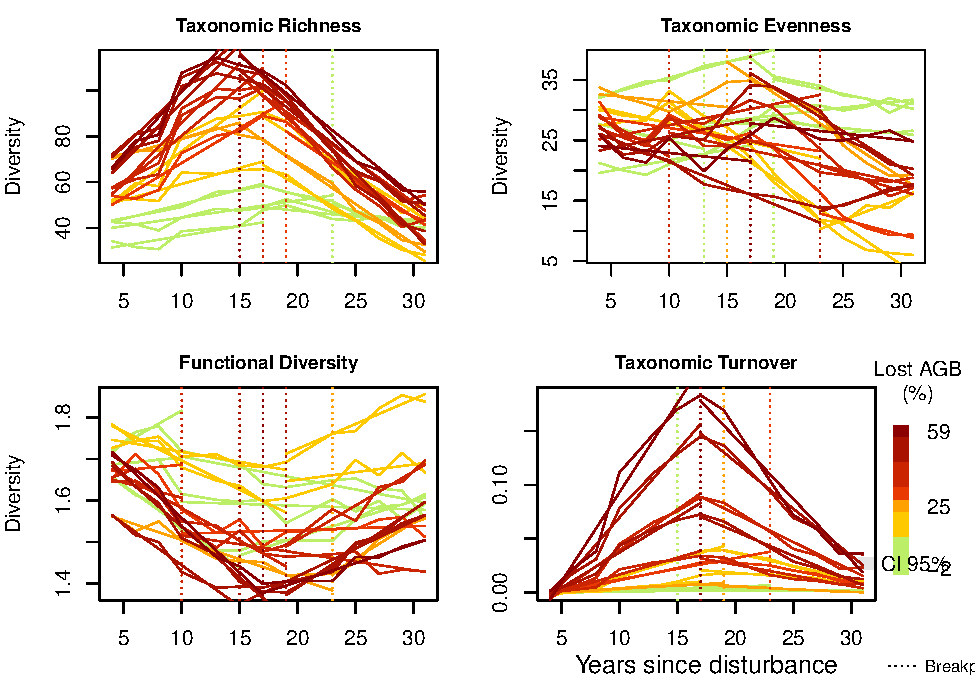
\includegraphics{RecruitmentTrajectories_SuppMat_files/figure-latex/BPanalysis-1} 

}

\caption{Figure S1: Breakpoint analysis of post-disturbance trajectories regarding, from left to right, taxonomic richness, taxonomic evenness, functional diversity, and taxonomic turnver of 2-years laps recuited communities. The best linear models segmented according to break points are selected based on their mean square errors. Dots are the observed trajectories, plain lines are linera model, and vertical dotted lines are the break points. Lines color correspond to initial disturbance intensity.}\label{fig:BPanalysis}
\end{figure}

\begin{table*}[t]

\caption{\label{tab:Splist}Table S2: List of recruited species for all plots throughout the 30 years inventoried.}
\begin{tabular}{lll}
\toprule
\textbf{Famille} & \textbf{Genre} & \textbf{Espece}\\
\midrule
\em{Anacardiaceae} & \em{Anacardium} & \em{spruceanum}\\
\em{Anacardiaceae} & \em{Tapirira} & \em{bethanniana}\\
\em{Anacardiaceae} & \em{Tapirira} & \em{guianensis}\\
\em{Anacardiaceae} & \em{Tapirira} & \em{obtusa}\\
\em{Anacardiaceae} & \em{Thyrsodium} & \em{guianense}\\
\addlinespace
\em{Anacardiaceae} & \em{Thyrsodium} & \em{puberulum}\\
\em{Anacardiaceae} & \em{Thyrsodium} & \em{spruceanum}\\
\em{Annonaceae} & \em{Anaxagorea} & \em{acuminata}\\
\em{Annonaceae} & \em{Anaxagorea} & \em{dolichocarpa}\\
\em{Annonaceae} & \em{Annona} & \em{ambotay}\\
\addlinespace
\em{Annonaceae} & \em{Annona} & \em{exsucca}\\
\em{Annonaceae} & \em{Annona} & \em{foetida}\\
\em{Annonaceae} & \em{Annona} & \em{prevostiae}\\
\em{Annonaceae} & \em{Duguetia} & \em{calycina}\\
\em{Annonaceae} & \em{Duguetia} & \em{yeshidan}\\
\addlinespace
\em{Annonaceae} & \em{Fusaea} & \em{longifolia}\\
\em{Annonaceae} & \em{Guatteria} & \em{citriodora}\\
\em{Annonaceae} & \em{Guatteria} & \em{guianensis}\\
\em{Annonaceae} & \em{Guatteria} & \em{punctata}\\
\em{Annonaceae} & \em{Guatteria} & \em{schomburgkiana}\\
\addlinespace
\em{Annonaceae} & \em{Oxandra} & \em{asbeckii}\\
\em{Annonaceae} & \em{Unonopsis} & \em{rufescens}\\
\em{Annonaceae} & \em{Xylopia} & \em{aromatica}\\
\em{Annonaceae} & \em{Xylopia} & \em{cayennensis}\\
\em{Annonaceae} & \em{Xylopia} & \em{crinita}\\
\addlinespace
\em{Annonaceae} & \em{Xylopia} & \em{frutescens}\\
\em{Annonaceae} & \em{Xylopia} & \em{nitida}\\
\em{Annonaceae} & \em{Xylopia} & \em{pulcherrima}\\
\em{Annonaceae} & \em{Xylopia} & \em{surinamensis}\\
\em{Apocynaceae} & \em{Ambelania} & \em{acida}\\
\addlinespace
\em{Apocynaceae} & \em{Aspidosperma} & \em{album}\\
\em{Apocynaceae} & \em{Aspidosperma} & \em{desmanthum}\\
\em{Apocynaceae} & \em{Aspidosperma} & \em{excelsum}\\
\em{Apocynaceae} & \em{Aspidosperma} & \em{helstonei}\\
\em{Apocynaceae} & \em{Aspidosperma} & \em{oblongum}\\
\addlinespace
\em{Apocynaceae} & \em{Aspidosperma} & \em{spruceanum}\\
\em{Apocynaceae} & \em{Couma} & \em{guianensis}\\
\em{Apocynaceae} & \em{Himatanthus} & \em{articulatus}\\
\em{Apocynaceae} & \em{Himatanthus} & \em{bracteatus}\\
\em{Apocynaceae} & \em{Lacmellea} & \em{aculeata}\\
\addlinespace
\em{Apocynaceae} & \em{Macoubea} & \em{guianensis}\\
\em{Apocynaceae} & \em{Parahancornia} & \em{fasciculata}\\
\em{Apocynaceae} & \em{Rauvolfia} & \em{paraensis}\\
\em{Apocynaceae} & \em{Tabernaemontana} & \em{attenuata}\\
\em{Aquifoliaceae} & \em{Ilex} & \em{inundata}\\
\addlinespace
\em{Aquifoliaceae} & \em{Ilex} & \em{sp.2CAY-ATDN}\\
\em{Araliaceae} & \em{Schefflera} & \em{decaphylla}\\
\em{Arecaceae} & \em{Astrocaryum} & \em{sciophilum}\\
\em{Arecaceae} & \em{Attalea} & \em{maripa}\\
\em{Arecaceae} & \em{Euterpe} & \em{oleracea}\\
\addlinespace
\em{Arecaceae} & \em{Oenocarpus} & \em{bacaba}\\
\em{Arecaceae} & \em{Oenocarpus} & \em{bataua}\\
\em{Arecaceae} & \em{Socratea} & \em{exorrhiza}\\
\em{Arecaceae} & \em{Syagrus} & \em{inajai}\\
\em{Bignoniaceae} & \em{Handroanthus} & \em{serratifolius}\\
\addlinespace
\em{Bignoniaceae} & \em{Jacaranda} & \em{copaia}\\
\em{Bignoniaceae} & \em{Tabebuia} & \em{insignis}\\
\em{Boraginaceae} & \em{Cordia} & \em{exaltata}\\
\em{Boraginaceae} & \em{Cordia} & \em{goeldiana}\\
\em{Boraginaceae} & \em{Cordia} & \em{nervosa}\\
\addlinespace
\em{Boraginaceae} & \em{Cordia} & \em{panicularis}\\
\em{Boraginaceae} & \em{Cordia} & \em{sagotii}\\
\em{Boraginaceae} & \em{Cordia} & \em{sprucei}\\
\em{Boraginaceae} & \em{Cordia} & \em{toqueve}\\
\em{Burseraceae} & \em{Dacryodes} & \em{nitens}\\
\addlinespace
\em{Burseraceae} & \em{Dacryodes} & \em{sp.4CAY-ATDN}\\
\em{Burseraceae} & \em{Protium} & \em{apiculatum}\\
\em{Burseraceae} & \em{Protium} & \em{decandrum}\\
\em{Burseraceae} & \em{Protium} & \em{gallicum}\\
\em{Burseraceae} & \em{Protium} & \em{giganteum}\\
\addlinespace
\em{Burseraceae} & \em{Protium} & \em{guianense}\\
\em{Burseraceae} & \em{Protium} & \em{opacum}\\
\em{Burseraceae} & \em{Protium} & \em{plagiocarpium}\\
\em{Burseraceae} & \em{Protium} & \em{sagotianum}\\
\em{Burseraceae} & \em{Protium} & \em{subserratum}\\
\addlinespace
\em{Burseraceae} & \em{Protium} & \em{tenuifolium}\\
\em{Burseraceae} & \em{Protium} & \em{trifoliolatum}\\
\em{Burseraceae} & \em{Tetragastris} & \em{altissima}\\
\em{Burseraceae} & \em{Tetragastris} & \em{hostmannii}\\
\em{Burseraceae} & \em{Tetragastris} & \em{panamensis}\\
\addlinespace
\em{Burseraceae} & \em{Trattinnickia} & \em{burserifolia}\\
\em{Burseraceae} & \em{Trattinnickia} & \em{demerarae}\\
\em{Burseraceae} & \em{Trattinnickia} & \em{rhoifolia}\\
\em{Calophyllaceae} & \em{Caraipa} & \em{densifolia}\\
\em{Calophyllaceae} & \em{Caraipa} & \em{racemosa}\\
\addlinespace
\em{Calophyllaceae} & \em{Mahurea} & \em{palustris}\\
\em{Capparaceae} & \em{Capparidastrum} & \em{frondosum}\\
\em{Capparaceae} & \em{Neocalyptrocalyx} & \em{leprieurii}\\
\em{Cardiopteridaceae} & \em{Dendrobangia} & \em{boliviana}\\
\em{Caryocaraceae} & \em{Caryocar} & \em{glabrum}\\
\addlinespace
\em{Caryocaraceae} & \em{Caryocar} & \em{microcarpum}\\
\em{Celastraceae} & \em{Cheiloclinium} & \em{cognatum}\\
\em{Celastraceae} & \em{Hippocratea} & \em{volubilis}\\
\em{Celastraceae} & \em{Maytenus} & \em{guyanensis}\\
\em{Celastraceae} & \em{Maytenus} & \em{oblongata}\\
\addlinespace
\em{Celastraceae} & \em{Maytenus} & \em{sp.7CAY-ATDN}\\
\em{Chrysobalanaceae} & \em{Couepia} & \em{bracteosa}\\
\em{Chrysobalanaceae} & \em{Couepia} & \em{caryophylloides}\\
\em{Chrysobalanaceae} & \em{Couepia} & \em{guianensis}\\
\em{Chrysobalanaceae} & \em{Couepia} & \em{habrantha}\\
\addlinespace
\em{Chrysobalanaceae} & \em{Couepia} & \em{magnoliifolia}\\
\em{Chrysobalanaceae} & \em{Couepia} & \em{obovata}\\
\em{Chrysobalanaceae} & \em{Couepia} & \em{parillo}\\
\em{Chrysobalanaceae} & \em{Gaulettia} & \em{parillo}\\
\em{Chrysobalanaceae} & \em{Hirtella} & \em{bicornis}\\
\addlinespace
\em{Chrysobalanaceae} & \em{Hirtella} & \em{glandulosa}\\
\em{Chrysobalanaceae} & \em{Hirtella} & \em{hispidula}\\
\em{Chrysobalanaceae} & \em{Licania} & \em{alba}\\
\em{Chrysobalanaceae} & \em{Licania} & \em{canescens}\\
\em{Chrysobalanaceae} & \em{Licania} & \em{densiflora}\\
\addlinespace
\em{Chrysobalanaceae} & \em{Licania} & \em{granvillei}\\
\em{Chrysobalanaceae} & \em{Licania} & \em{heteromorpha}\\
\em{Chrysobalanaceae} & \em{Licania} & \em{hypoleuca}\\
\em{Chrysobalanaceae} & \em{Licania} & \em{latifolia}\\
\em{Chrysobalanaceae} & \em{Licania} & \em{latistipula}\\
\addlinespace
\em{Chrysobalanaceae} & \em{Licania} & \em{laxiflora}\\
\em{Chrysobalanaceae} & \em{Licania} & \em{licaniiflora}\\
\em{Chrysobalanaceae} & \em{Licania} & \em{longistyla}\\
\em{Chrysobalanaceae} & \em{Licania} & \em{majuscula}\\
\em{Chrysobalanaceae} & \em{Licania} & \em{membranacea}\\
\addlinespace
\em{Chrysobalanaceae} & \em{Licania} & \em{micrantha}\\
\em{Chrysobalanaceae} & \em{Licania} & \em{ovalifolia}\\
\em{Chrysobalanaceae} & \em{Licania} & \em{parvifructa}\\
\em{Chrysobalanaceae} & \em{Licania} & \em{robusta}\\
\em{Chrysobalanaceae} & \em{Licania} & \em{sprucei}\\
\addlinespace
\em{Chrysobalanaceae} & \em{Parinari} & \em{campestris}\\
\em{Chrysobalanaceae} & \em{Parinari} & \em{montana}\\
\em{Chrysobalanaceae} & \em{Parinari} & \em{parvifolia}\\
\em{Chrysobalanaceae} & \em{Parinari} & \em{rodolphii}\\
\em{Chrysobalanaceae} & \em{Indet.} & \em{sp.1CAY-ATDN}\\
\addlinespace
\em{Clusiaceae} & \em{Clusia} & \em{grandiflora}\\
\em{Clusiaceae} & \em{Garcinia} & \em{benthamiana}\\
\em{Clusiaceae} & \em{Garcinia} & \em{madruno}\\
\em{Clusiaceae} & \em{Moronobea} & \em{coccinea}\\
\em{Clusiaceae} & \em{Platonia} & \em{insignis}\\
\addlinespace
\em{Clusiaceae} & \em{Symphonia} & \em{globulifera}\\
\em{Clusiaceae} & \em{Symphonia} & \em{sp.1}\\
\em{Clusiaceae} & \em{Tovomita} & \em{brevistaminea}\\
\em{Clusiaceae} & \em{Tovomita} & \em{macrophylla}\\
\em{Clusiaceae} & \em{Tovomita} & \em{obovata}\\
\addlinespace
\em{Clusiaceae} & \em{Tovomita} & \em{sp.1}\\
\em{Clusiaceae} & \em{Tovomita} & \em{sp.10CAY-ATDN}\\
\em{Clusiaceae} & \em{Tovomita} & \em{sp.11CAY-ATDN}\\
\em{Clusiaceae} & \em{Tovomita} & \em{sp.2}\\
\em{Clusiaceae} & \em{Tovomita} & \em{sp.22CAY-ATDN}\\
\addlinespace
\em{Clusiaceae} & \em{Tovomita} & \em{sp.2CAY-ATDN}\\
\em{Clusiaceae} & \em{Tovomita} & \em{sp.3CAY-ATDN}\\
\em{Clusiaceae} & \em{Tovomita} & \em{sp.5CAY-ATDN}\\
\em{Clusiaceae} & \em{Tovomita} & \em{sp.9CAY-ATDN}\\
\em{Clusiaceae} & \em{Tovomita} & \em{sp.B1}\\
\addlinespace
\em{Combretaceae} & \em{Buchenavia} & \em{grandis}\\
\em{Combretaceae} & \em{Buchenavia} & \em{guianensis}\\
\em{Combretaceae} & \em{Buchenavia} & \em{nitidissima}\\
\em{Combretaceae} & \em{Buchenavia} & \em{tetraphylla}\\
\em{Combretaceae} & \em{Terminalia} & \em{amazonia}\\
\addlinespace
\em{Convolvulaceae} & \em{Dicranostyles} & \em{integra}\\
\em{Dichapetalaceae} & \em{Tapura} & \em{amazonica}\\
\em{Dichapetalaceae} & \em{Tapura} & \em{capitulifera}\\
\em{Dilleniaceae} & \em{Doliocarpus} & \em{sp.1}\\
\em{Ebenaceae} & \em{Diospyros} & \em{capreifolia}\\
\addlinespace
\em{Ebenaceae} & \em{Diospyros} & \em{carbonaria}\\
\em{Ebenaceae} & \em{Diospyros} & \em{guianensis}\\
\em{Ebenaceae} & \em{Diospyros} & \em{vestita}\\
\em{Elaeocarpaceae} & \em{Sloanea} & \em{brevipes}\\
\em{Elaeocarpaceae} & \em{Sloanea} & \em{garckeana}\\
\addlinespace
\em{Elaeocarpaceae} & \em{Sloanea} & \em{grandiflora}\\
\em{Elaeocarpaceae} & \em{Sloanea} & \em{guianensis}\\
\em{Elaeocarpaceae} & \em{Sloanea} & \em{latifolia}\\
\em{Elaeocarpaceae} & \em{Sloanea} & \em{latifolia\_form2}\\
\em{Elaeocarpaceae} & \em{Sloanea} & \em{laxiflora}\\
\addlinespace
\em{Elaeocarpaceae} & \em{Sloanea} & \em{parviflora}\\
\em{Elaeocarpaceae} & \em{Sloanea} & \em{sinemariensis}\\
\em{Elaeocarpaceae} & \em{Sloanea} & \em{sp.1}\\
\em{Elaeocarpaceae} & \em{Sloanea} & \em{sp.14CAY-ATDN}\\
\em{Elaeocarpaceae} & \em{Sloanea} & \em{sp.17CAY-ATDN}\\
\addlinespace
\em{Elaeocarpaceae} & \em{Sloanea} & \em{sp.20CAY-ATDN}\\
\em{Elaeocarpaceae} & \em{Sloanea} & \em{sp.21CAY-ATDN}\\
\em{Elaeocarpaceae} & \em{Sloanea} & \em{sp.22CAY-ATDN}\\
\em{Elaeocarpaceae} & \em{Sloanea} & \em{sp.24CAY-ATDN}\\
\em{Elaeocarpaceae} & \em{Sloanea} & \em{sp.2CAY-ATDN}\\
\addlinespace
\em{Elaeocarpaceae} & \em{Sloanea} & \em{sp.4CAY-ATDN}\\
\em{Elaeocarpaceae} & \em{Sloanea} & \em{sp.5CAY-ATDN}\\
\em{Elaeocarpaceae} & \em{Sloanea} & \em{sp.8CAY-ATDN}\\
\em{Elaeocarpaceae} & \em{Sloanea} & \em{sp.P33}\\
\em{Elaeocarpaceae} & \em{Sloanea} & \em{tuerckheimii}\\
\addlinespace
\em{Emmotaceae} & \em{Emmotum} & \em{fagifolium}\\
\em{Erythroxylaceae} & \em{Erythroxylum} & \em{citrifolium}\\
\em{Erythroxylaceae} & \em{Erythroxylum} & \em{ligustrinum}\\
\em{Erythroxylaceae} & \em{Erythroxylum} & \em{lineolatum}\\
\em{Erythroxylaceae} & \em{Erythroxylum} & \em{sp.1CAY-ATDN}\\
\addlinespace
\em{Euphorbiaceae} & \em{Alchornea} & \em{discolor}\\
\em{Euphorbiaceae} & \em{Alchornea} & \em{triplinervia}\\
\em{Euphorbiaceae} & \em{Alchorneopsis} & \em{floribunda}\\
\em{Euphorbiaceae} & \em{Chaetocarpus} & \em{schomburgkianus}\\
\em{Euphorbiaceae} & \em{Chaetocarpus} & \em{sp.1CAY-ATDN}\\
\addlinespace
\em{Euphorbiaceae} & \em{Conceveiba} & \em{guianensis}\\
\em{Euphorbiaceae} & \em{Glycydendron} & \em{amazonicum}\\
\em{Euphorbiaceae} & \em{Hevea} & \em{guianensis}\\
\em{Euphorbiaceae} & \em{Mabea} & \em{piriri}\\
\em{Euphorbiaceae} & \em{Pera} & \em{glabrata}\\
\addlinespace
\em{Euphorbiaceae} & \em{Pogonophora} & \em{schomburgkiana}\\
\em{Euphorbiaceae} & \em{Sagotia} & \em{racemosa}\\
\em{Euphorbiaceae} & \em{Sandwithia} & \em{guyanensis}\\
\em{Euphorbiaceae} & \em{Indet.} & \em{sp.P4}\\
\em{Fabaceae} & \em{Abarema} & \em{jupunba}\\
\addlinespace
\em{Fabaceae} & \em{Abarema} & \em{mataybifolia}\\
\em{Fabaceae} & \em{Albizia} & \em{pedicellaris}\\
\em{Fabaceae} & \em{Alexa} & \em{wachenheimii}\\
\em{Fabaceae} & \em{Andira} & \em{coriacea}\\
\em{Fabaceae} & \em{Bocoa} & \em{prouacensis}\\
\addlinespace
\em{Fabaceae} & \em{Cassia} & \em{spruceana}\\
\em{Fabaceae} & \em{Copaifera} & \em{guianensis}\\
\em{Fabaceae} & \em{Dialium} & \em{guianense}\\
\em{Fabaceae} & \em{Dicorynia} & \em{guianensis}\\
\em{Fabaceae} & \em{Dimorphandra} & \em{polyandra}\\
\addlinespace
\em{Fabaceae} & \em{Diplotropis} & \em{purpurea}\\
\em{Fabaceae} & \em{Dipteryx} & \em{odorata}\\
\em{Fabaceae} & \em{Enterolobium} & \em{oldemanii}\\
\em{Fabaceae} & \em{Enterolobium} & \em{schomburgkii}\\
\em{Fabaceae} & \em{Enterolobium} & \em{sp.1CAY-ATDN}\\
\addlinespace
\em{Fabaceae} & \em{Eperua} & \em{falcata}\\
\em{Fabaceae} & \em{Eperua} & \em{grandiflora}\\
\em{Fabaceae} & \em{Eperua} & \em{rubiginosa}\\
\em{Fabaceae} & \em{Hymenolobium} & \em{flavum}\\
\em{Fabaceae} & \em{Inga} & \em{acreana}\\
\addlinespace
\em{Fabaceae} & \em{Inga} & \em{acrocephala}\\
\em{Fabaceae} & \em{Inga} & \em{alba}\\
\em{Fabaceae} & \em{Inga} & \em{brachystachys}\\
\em{Fabaceae} & \em{Inga} & \em{brevipes}\\
\em{Fabaceae} & \em{Inga} & \em{capitata}\\
\addlinespace
\em{Fabaceae} & \em{Inga} & \em{capitata\_form2}\\
\em{Fabaceae} & \em{Inga} & \em{cayennensis}\\
\em{Fabaceae} & \em{Inga} & \em{cordatoalata}\\
\em{Fabaceae} & \em{Inga} & \em{cylindrica}\\
\em{Fabaceae} & \em{Inga} & \em{disticha}\\
\addlinespace
\em{Fabaceae} & \em{Inga} & \em{fanchoniana}\\
\em{Fabaceae} & \em{Inga} & \em{graciliflora}\\
\em{Fabaceae} & \em{Inga} & \em{gracilifolia}\\
\em{Fabaceae} & \em{Inga} & \em{jenmanii}\\
\em{Fabaceae} & \em{Inga} & \em{lomatophylla}\\
\addlinespace
\em{Fabaceae} & \em{Inga} & \em{longipedunculata}\\
\em{Fabaceae} & \em{Inga} & \em{loubryana}\\
\em{Fabaceae} & \em{Inga} & \em{marginata}\\
\em{Fabaceae} & \em{Inga} & \em{melinonis}\\
\em{Fabaceae} & \em{Inga} & \em{nobilis}\\
\addlinespace
\em{Fabaceae} & \em{Inga} & \em{nouragensis}\\
\em{Fabaceae} & \em{Inga} & \em{paraensis}\\
\em{Fabaceae} & \em{Inga} & \em{pezizifera}\\
\em{Fabaceae} & \em{Inga} & \em{rubiginosa}\\
\em{Fabaceae} & \em{Inga} & \em{sarmentosa}\\
\addlinespace
\em{Fabaceae} & \em{Inga} & \em{sp.12CAY-ATDN}\\
\em{Fabaceae} & \em{Inga} & \em{sp.16CAY-ATDN}\\
\em{Fabaceae} & \em{Inga} & \em{sp.18CAY-ATDN}\\
\em{Fabaceae} & \em{Inga} & \em{sp.4}\\
\em{Fabaceae} & \em{Inga} & \em{splendens}\\
\addlinespace
\em{Fabaceae} & \em{Inga} & \em{stipularis}\\
\em{Fabaceae} & \em{Inga} & \em{thibaudiana}\\
\em{Fabaceae} & \em{Inga} & \em{tubiformis}\\
\em{Fabaceae} & \em{Inga} & \em{umbellifera}\\
\em{Fabaceae} & \em{Inga} & \em{virgultosa}\\
\addlinespace
\em{Fabaceae} & \em{Macrolobium} & \em{bifolium}\\
\em{Fabaceae} & \em{Mimosa} & \em{guilandinae}\\
\em{Fabaceae} & \em{Ormosia} & \em{bolivarensis}\\
\em{Fabaceae} & \em{Ormosia} & \em{coccinea}\\
\em{Fabaceae} & \em{Ormosia} & \em{coutinhoi}\\
\addlinespace
\em{Fabaceae} & \em{Ormosia} & \em{melanocarpa}\\
\em{Fabaceae} & \em{Ormosia} & \em{paraensis}\\
\em{Fabaceae} & \em{Ormosia} & \em{stipularis}\\
\em{Fabaceae} & \em{Parkia} & \em{gigantocarpa}\\
\em{Fabaceae} & \em{Parkia} & \em{nitida}\\
\addlinespace
\em{Fabaceae} & \em{Parkia} & \em{pendula}\\
\em{Fabaceae} & \em{Parkia} & \em{ulei}\\
\em{Fabaceae} & \em{Parkia} & \em{velutina}\\
\em{Fabaceae} & \em{Peltogyne} & \em{paniculata}\\
\em{Fabaceae} & \em{Peltogyne} & \em{sp.1CAY-ATDN}\\
\addlinespace
\em{Fabaceae} & \em{Peltogyne} & \em{sp.2CAY-ATDN}\\
\em{Fabaceae} & \em{Platymiscium} & \em{pinnatum}\\
\em{Fabaceae} & \em{Poecilanthe} & \em{effusa}\\
\em{Fabaceae} & \em{Poecilanthe} & \em{hostmannii}\\
\em{Fabaceae} & \em{Pseudopiptadenia} & \em{psilostachya}\\
\addlinespace
\em{Fabaceae} & \em{Pterocarpus} & \em{officinalis}\\
\em{Fabaceae} & \em{Pterocarpus} & \em{rohrii}\\
\em{Fabaceae} & \em{Recordoxylon} & \em{speciosum}\\
\em{Fabaceae} & \em{Stryphnodendron} & \em{polystachyum}\\
\em{Fabaceae} & \em{Stryphnodendron} & \em{sp.3CAY-ATDN}\\
\addlinespace
\em{Fabaceae} & \em{Swartzia} & \em{arborescens}\\
\em{Fabaceae} & \em{Swartzia} & \em{benthamiana}\\
\em{Fabaceae} & \em{Swartzia} & \em{grandifolia}\\
\em{Fabaceae} & \em{Swartzia} & \em{guianensis}\\
\em{Fabaceae} & \em{Swartzia} & \em{leblondii}\\
\addlinespace
\em{Fabaceae} & \em{Swartzia} & \em{oblanceolata}\\
\em{Fabaceae} & \em{Swartzia} & \em{panacoco}\\
\em{Fabaceae} & \em{Swartzia} & \em{polyphylla}\\
\em{Fabaceae} & \em{Tachigali} & \em{guianensis}\\
\em{Fabaceae} & \em{Tachigali} & \em{melinonii}\\
\addlinespace
\em{Fabaceae} & \em{Tachigali} & \em{paraensis}\\
\em{Fabaceae} & \em{Tachigali} & \em{richardiana}\\
\em{Fabaceae} & \em{Tachigali} & \em{sp.1}\\
\em{Fabaceae} & \em{Tachigali} & \em{sp.5CAY-ATDN}\\
\em{Fabaceae} & \em{Vatairea} & \em{erythrocarpa}\\
\addlinespace
\em{Fabaceae} & \em{Vatairea} & \em{paraensis}\\
\em{Fabaceae} & \em{Vataireopsis} & \em{surinamensis}\\
\em{Fabaceae} & \em{Vouacapoua} & \em{americana}\\
\em{Fabaceae} & \em{Zygia} & \em{tetragona}\\
\em{Goupiaceae} & \em{Goupia} & \em{glabra}\\
\addlinespace
\em{Humiriaceae} & \em{Humiria} & \em{balsamifera}\\
\em{Humiriaceae} & \em{Humiriastrum} & \em{excelsum}\\
\em{Humiriaceae} & \em{Humiriastrum} & \em{subcrenatum}\\
\em{Humiriaceae} & \em{Sacoglottis} & \em{cydonioides}\\
\em{Humiriaceae} & \em{Sacoglottis} & \em{guianensis}\\
\addlinespace
\em{Humiriaceae} & \em{Vantanea} & \em{guianensis}\\
\em{Humiriaceae} & \em{Vantanea} & \em{parviflora}\\
\em{Hypericaceae} & \em{Vismia} & \em{cayennensis}\\
\em{Hypericaceae} & \em{Vismia} & \em{guianensis}\\
\em{Hypericaceae} & \em{Vismia} & \em{latifolia}\\
\addlinespace
\em{Hypericaceae} & \em{Vismia} & \em{ramuliflora}\\
\em{Hypericaceae} & \em{Vismia} & \em{sessilifolia}\\
\em{Hypericaceae} & \em{Vismia} & \em{sp.1Guyafor}\\
\em{Hypericaceae} & \em{Vismia} & \em{sp.P1}\\
\em{Icacinaceae} & \em{Poraqueiba} & \em{guianensis}\\
\addlinespace
\em{Lacistemataceae} & \em{Lacistema} & \em{aggregatum}\\
\em{Lacistemataceae} & \em{Lacistema} & \em{grandifolium}\\
\em{Lacistemataceae} & \em{Lacistema} & \em{polystachyum}\\
\em{Lamiaceae} & \em{Vitex} & \em{guianensis}\\
\em{Lamiaceae} & \em{Vitex} & \em{triflora}\\
\addlinespace
\em{Lauraceae} & \em{Aniba} & \em{citrifolia}\\
\em{Lauraceae} & \em{Aniba} & \em{guianensis}\\
\em{Lauraceae} & \em{Aniba} & \em{rosaeodora}\\
\em{Lauraceae} & \em{Aniba} & \em{taubertiana}\\
\em{Lauraceae} & \em{Aniba} & \em{williamsii}\\
\addlinespace
\em{Lauraceae} & \em{Endlicheria} & \em{melinonii}\\
\em{Lauraceae} & \em{Licaria} & \em{cannella}\\
\em{Lauraceae} & \em{Licaria} & \em{chrysophylla}\\
\em{Lauraceae} & \em{Licaria} & \em{debilis}\\
\em{Lauraceae} & \em{Licaria} & \em{guianensis}\\
\addlinespace
\em{Lauraceae} & \em{Licaria} & \em{martiniana}\\
\em{Lauraceae} & \em{Mezilaurus} & \em{sp.1CAY-ATDN}\\
\em{Lauraceae} & \em{Nectandra} & \em{globosa}\\
\em{Lauraceae} & \em{Ocotea} & \em{amazonica}\\
\em{Lauraceae} & \em{Ocotea} & \em{argyrophylla}\\
\addlinespace
\em{Lauraceae} & \em{Ocotea} & \em{cernua}\\
\em{Lauraceae} & \em{Ocotea} & \em{cinerea}\\
\em{Lauraceae} & \em{Ocotea} & \em{glomerata}\\
\em{Lauraceae} & \em{Ocotea} & \em{nigra}\\
\em{Lauraceae} & \em{Ocotea} & \em{oblonga}\\
\addlinespace
\em{Lauraceae} & \em{Ocotea} & \em{percurrens}\\
\em{Lauraceae} & \em{Ocotea} & \em{puberula}\\
\em{Lauraceae} & \em{Ocotea} & \em{splendens}\\
\em{Lauraceae} & \em{Ocotea} & \em{subterminalis}\\
\em{Lauraceae} & \em{Ocotea} & \em{tomentella}\\
\addlinespace
\em{Lauraceae} & \em{Rhodostemonodaphne} & \em{grandis}\\
\em{Lauraceae} & \em{Rhodostemonodaphne} & \em{kunthiana}\\
\em{Lauraceae} & \em{Rhodostemonodaphne} & \em{morii}\\
\em{Lauraceae} & \em{Rhodostemonodaphne} & \em{rufovirgata}\\
\em{Lauraceae} & \em{Sextonia} & \em{rubra}\\
\addlinespace
\em{Lauraceae} & \em{Indet.} & \em{sp.30CAY-ATDN}\\
\em{Lauraceae} & \em{Indet.} & \em{sp.34CAY-ATDN}\\
\em{Lauraceae} & \em{Indet.} & \em{sp.38Guyafor}\\
\em{Lauraceae} & \em{Indet.} & \em{sp.39Guyafor}\\
\em{Lauraceae} & \em{Indet.} & \em{sp.B7}\\
\addlinespace
\em{Lecythidaceae} & \em{Couratari} & \em{calycina}\\
\em{Lecythidaceae} & \em{Couratari} & \em{gloriosa}\\
\em{Lecythidaceae} & \em{Couratari} & \em{guianensis}\\
\em{Lecythidaceae} & \em{Couratari} & \em{multiflora}\\
\em{Lecythidaceae} & \em{Couratari} & \em{oblongifolia}\\
\addlinespace
\em{Lecythidaceae} & \em{Eschweilera} & \em{collina}\\
\em{Lecythidaceae} & \em{Eschweilera} & \em{congestiflora}\\
\em{Lecythidaceae} & \em{Eschweilera} & \em{coriacea}\\
\em{Lecythidaceae} & \em{Eschweilera} & \em{decolorans}\\
\em{Lecythidaceae} & \em{Eschweilera} & \em{grandiflora}\\
\addlinespace
\em{Lecythidaceae} & \em{Eschweilera} & \em{grandiflora\_form2}\\
\em{Lecythidaceae} & \em{Eschweilera} & \em{parviflora}\\
\em{Lecythidaceae} & \em{Eschweilera} & \em{pedicellata}\\
\em{Lecythidaceae} & \em{Eschweilera} & \em{sagotiana}\\
\em{Lecythidaceae} & \em{Eschweilera} & \em{simiorum}\\
\addlinespace
\em{Lecythidaceae} & \em{Eschweilera} & \em{wachenheimii}\\
\em{Lecythidaceae} & \em{Gustavia} & \em{augusta}\\
\em{Lecythidaceae} & \em{Gustavia} & \em{hexapetala}\\
\em{Lecythidaceae} & \em{Lecythis} & \em{chartacea}\\
\em{Lecythidaceae} & \em{Lecythis} & \em{corrugata}\\
\addlinespace
\em{Lecythidaceae} & \em{Lecythis} & \em{corrugata subsp. corrugata}\\
\em{Lecythidaceae} & \em{Lecythis} & \em{holcogyne}\\
\em{Lecythidaceae} & \em{Lecythis} & \em{idatimon}\\
\em{Lecythidaceae} & \em{Lecythis} & \em{persistens}\\
\em{Lecythidaceae} & \em{Lecythis} & \em{poiteaui}\\
\addlinespace
\em{Lecythidaceae} & \em{Lecythis} & \em{zabucajo}\\
\em{Lecythidaceae} & \em{Indet.} & \em{sp.6Guyafor}\\
\em{Lecythidaceae} & \em{Indet.} & \em{sp.7Guyafor}\\
\em{Lecythidaceae} & \em{Indet.} & \em{sp.8Guyafor}\\
\em{Linaceae} & \em{Hebepetalum} & \em{humiriifolium}\\
\addlinespace
\em{Loganiaceae} & \em{Antonia} & \em{ovata}\\
\em{Malpighiaceae} & \em{Byrsonima} & \em{aerugo}\\
\em{Malpighiaceae} & \em{Byrsonima} & \em{densa}\\
\em{Malpighiaceae} & \em{Byrsonima} & \em{laevigata}\\
\em{Malvaceae} & \em{Apeiba} & \em{glabra}\\
\addlinespace
\em{Malvaceae} & \em{Apeiba} & \em{petoumo}\\
\em{Malvaceae} & \em{Catostemma} & \em{fragrans}\\
\em{Malvaceae} & \em{Eriotheca} & \em{globosa}\\
\em{Malvaceae} & \em{Eriotheca} & \em{longitubulosa}\\
\em{Malvaceae} & \em{Luehea} & \em{speciosa}\\
\addlinespace
\em{Malvaceae} & \em{Lueheopsis} & \em{rugosa}\\
\em{Malvaceae} & \em{Pachira} & \em{dolichocalyx}\\
\em{Malvaceae} & \em{Pachira} & \em{insignis}\\
\em{Malvaceae} & \em{Sterculia} & \em{excelsa}\\
\em{Malvaceae} & \em{Sterculia} & \em{multiovula}\\
\addlinespace
\em{Malvaceae} & \em{Sterculia} & \em{pruriens}\\
\em{Malvaceae} & \em{Sterculia} & \em{sp.P1}\\
\em{Malvaceae} & \em{Sterculia} & \em{speciosa}\\
\em{Malvaceae} & \em{Theobroma} & \em{subincanum}\\
\em{Malvaceae} & \em{Theobroma} & \em{velutinum}\\
\addlinespace
\em{Melastomataceae} & \em{Bellucia} & \em{grossularioides}\\
\em{Melastomataceae} & \em{Henriettea} & \em{succosa}\\
\em{Melastomataceae} & \em{Henriettella} & \em{flavescens}\\
\em{Melastomataceae} & \em{Loreya} & \em{arborescens}\\
\em{Melastomataceae} & \em{Loreya} & \em{mespiloides}\\
\addlinespace
\em{Melastomataceae} & \em{Miconia} & \em{acuminata}\\
\em{Melastomataceae} & \em{Miconia} & \em{argyrophylla}\\
\em{Melastomataceae} & \em{Miconia} & \em{fragilis}\\
\em{Melastomataceae} & \em{Miconia} & \em{hypoleuca}\\
\em{Melastomataceae} & \em{Miconia} & \em{minutiflora}\\
\addlinespace
\em{Melastomataceae} & \em{Miconia} & \em{plukenetii}\\
\em{Melastomataceae} & \em{Miconia} & \em{poeppigii}\\
\em{Melastomataceae} & \em{Miconia} & \em{prasina}\\
\em{Melastomataceae} & \em{Miconia} & \em{ruficalyx}\\
\em{Melastomataceae} & \em{Miconia} & \em{trinervia}\\
\addlinespace
\em{Melastomataceae} & \em{Miconia} & \em{tschudyoides}\\
\em{Melastomataceae} & \em{Mouriri} & \em{angulicosta}\\
\em{Melastomataceae} & \em{Mouriri} & \em{crassifolia}\\
\em{Melastomataceae} & \em{Mouriri} & \em{dumetosa}\\
\em{Melastomataceae} & \em{Mouriri} & \em{huberi}\\
\addlinespace
\em{Melastomataceae} & \em{Mouriri} & \em{nervosa}\\
\em{Melastomataceae} & \em{Mouriri} & \em{sagotiana}\\
\em{Melastomataceae} & \em{Mouriri} & \em{sp.2CAY-ATDN}\\
\em{Melastomataceae} & \em{Votomita} & \em{guianensis}\\
\em{Meliaceae} & \em{Carapa} & \em{procera}\\
\addlinespace
\em{Meliaceae} & \em{Carapa} & \em{surinamensis}\\
\em{Meliaceae} & \em{Guarea} & \em{carinata}\\
\em{Meliaceae} & \em{Guarea} & \em{costata}\\
\em{Meliaceae} & \em{Guarea} & \em{glabra}\\
\em{Meliaceae} & \em{Guarea} & \em{kunthiana}\\
\addlinespace
\em{Meliaceae} & \em{Guarea} & \em{pubescens}\\
\em{Meliaceae} & \em{Trichilia} & \em{cipo}\\
\em{Meliaceae} & \em{Trichilia} & \em{micrantha}\\
\em{Meliaceae} & \em{Trichilia} & \em{schomburgkii}\\
\em{Moraceae} & \em{Bagassa} & \em{guianensis}\\
\addlinespace
\em{Moraceae} & \em{Brosimum} & \em{acutifolium}\\
\em{Moraceae} & \em{Brosimum} & \em{guianense}\\
\em{Moraceae} & \em{Brosimum} & \em{rubescens}\\
\em{Moraceae} & \em{Brosimum} & \em{utile}\\
\em{Moraceae} & \em{Ficus} & \em{americana}\\
\addlinespace
\em{Moraceae} & \em{Ficus} & \em{broadwayi}\\
\em{Moraceae} & \em{Ficus} & \em{gomelleira}\\
\em{Moraceae} & \em{Ficus} & \em{malacocarpa}\\
\em{Moraceae} & \em{Ficus} & \em{maroniensis}\\
\em{Moraceae} & \em{Ficus} & \em{nymphaeifolia}\\
\addlinespace
\em{Moraceae} & \em{Ficus} & \em{panurensis}\\
\em{Moraceae} & \em{Ficus} & \em{pertusa}\\
\em{Moraceae} & \em{Ficus} & \em{piresiana}\\
\em{Moraceae} & \em{Ficus} & \em{pulchella}\\
\em{Moraceae} & \em{Ficus} & \em{schumacheri}\\
\addlinespace
\em{Moraceae} & \em{Helicostylis} & \em{pedunculata}\\
\em{Moraceae} & \em{Helicostylis} & \em{tomentosa}\\
\em{Moraceae} & \em{Maquira} & \em{guianensis}\\
\em{Moraceae} & \em{Naucleopsis} & \em{glabra}\\
\em{Moraceae} & \em{Naucleopsis} & \em{guianensis}\\
\addlinespace
\em{Moraceae} & \em{Perebea} & \em{mollis}\\
\em{Moraceae} & \em{Perebea} & \em{rubra}\\
\em{Moraceae} & \em{Pseudolmedia} & \em{laevis}\\
\em{Moraceae} & \em{Trymatococcus} & \em{amazonicus}\\
\em{Moraceae} & \em{Trymatococcus} & \em{oligandrus}\\
\addlinespace
\em{Myristicaceae} & \em{Iryanthera} & \em{hostmannii}\\
\em{Myristicaceae} & \em{Iryanthera} & \em{sagotiana}\\
\em{Myristicaceae} & \em{Virola} & \em{michelii}\\
\em{Myristicaceae} & \em{Virola} & \em{sebifera}\\
\em{Myristicaceae} & \em{Virola} & \em{surinamensis}\\
\addlinespace
\em{Myrtaceae} & \em{Calycolpus} & \em{goetheanus}\\
\em{Myrtaceae} & \em{Eugenia} & \em{albicans}\\
\em{Myrtaceae} & \em{Eugenia} & \em{anastomosans}\\
\em{Myrtaceae} & \em{Eugenia} & \em{coffeifolia}\\
\em{Myrtaceae} & \em{Eugenia} & \em{cucullata}\\
\addlinespace
\em{Myrtaceae} & \em{Eugenia} & \em{cupulata}\\
\em{Myrtaceae} & \em{Eugenia} & \em{exaltata}\\
\em{Myrtaceae} & \em{Eugenia} & \em{latifolia}\\
\em{Myrtaceae} & \em{Eugenia} & \em{patens}\\
\em{Myrtaceae} & \em{Eugenia} & \em{patrisii}\\
\addlinespace
\em{Myrtaceae} & \em{Eugenia} & \em{pseudopsidium}\\
\em{Myrtaceae} & \em{Eugenia} & \em{sp.FG21-Holst}\\
\em{Myrtaceae} & \em{Eugenia} & \em{sp.FG9-Holst}\\
\em{Myrtaceae} & \em{Eugenia} & \em{tetramera}\\
\em{Myrtaceae} & \em{Myrcia} & \em{decorticans}\\
\addlinespace
\em{Myrtaceae} & \em{Myrcia} & \em{fallax}\\
\em{Myrtaceae} & \em{Myrcia} & \em{magnoliifolia}\\
\em{Myrtaceae} & \em{Myrciaria} & \em{floribunda}\\
\em{Myrtaceae} & \em{Indet.} & \em{sp.B1}\\
\em{Nyctaginaceae} & \em{Neea} & \em{sp.1CAY-ATDN}\\
\addlinespace
\em{Nyctaginaceae} & \em{Indet.} & \em{sp.4CAY-ATDN}\\
\em{Nyctaginaceae} & \em{Indet.} & \em{sp.7CAY-ATDN}\\
\em{Nyctaginaceae} & \em{Indet.} & \em{sp.P1}\\
\em{Ochnaceae} & \em{Elvasia} & \em{elvasioides}\\
\em{Ochnaceae} & \em{Lacunaria} & \em{crenata}\\
\addlinespace
\em{Ochnaceae} & \em{Lacunaria} & \em{jenmanii}\\
\em{Ochnaceae} & \em{Ouratea} & \em{decagyna}\\
\em{Ochnaceae} & \em{Ouratea} & \em{guianensis}\\
\em{Ochnaceae} & \em{Quiina} & \em{guianensis}\\
\em{Ochnaceae} & \em{Quiina} & \em{integrifolia}\\
\addlinespace
\em{Ochnaceae} & \em{Quiina} & \em{macrophylla}\\
\em{Ochnaceae} & \em{Quiina} & \em{obovata}\\
\em{Ochnaceae} & \em{Quiina} & \em{oiapocensis}\\
\em{Ochnaceae} & \em{Touroulia} & \em{guianensis}\\
\em{Olacaceae} & \em{Chaunochiton} & \em{kappleri}\\
\addlinespace
\em{Olacaceae} & \em{Heisteria} & \em{densifrons}\\
\em{Olacaceae} & \em{Heisteria} & \em{ovata}\\
\em{Olacaceae} & \em{Minquartia} & \em{guianensis}\\
\em{Opiliaceae} & \em{Agonandra} & \em{silvatica}\\
\em{Phyllanthaceae} & \em{Amanoa} & \em{congesta}\\
\addlinespace
\em{Phyllanthaceae} & \em{Amanoa} & \em{guianensis}\\
\em{Phyllanthaceae} & \em{Hieronyma} & \em{alchorneoides}\\
\em{Phyllanthaceae} & \em{Hieronyma} & \em{oblonga}\\
\em{Phyllanthaceae} & \em{Richeria} & \em{grandis}\\
\em{Polygonaceae} & \em{Coccoloba} & \em{mollis}\\
\addlinespace
\em{Primulaceae} & \em{Cybianthus} & \em{guyanensis}\\
\em{Primulaceae} & \em{Cybianthus} & \em{microbotrys}\\
\em{Proteaceae} & \em{Euplassa} & \em{pinnata}\\
\em{Proteaceae} & \em{Panopsis} & \em{sessilifolia}\\
\em{Putranjivaceae} & \em{Drypetes} & \em{fanshawei}\\
\addlinespace
\em{Putranjivaceae} & \em{Drypetes} & \em{variabilis}\\
\em{Rhizophoraceae} & \em{Cassipourea} & \em{guianensis}\\
\em{Rosaceae} & \em{Prunus} & \em{accumulans}\\
\em{Rosaceae} & \em{Prunus} & \em{myrtifolia}\\
\em{Rubiaceae} & \em{Amaioua} & \em{corymbosa}\\
\addlinespace
\em{Rubiaceae} & \em{Amaioua} & \em{guianensis}\\
\em{Rubiaceae} & \em{Chimarrhis} & \em{turbinata}\\
\em{Rubiaceae} & \em{Coussarea} & \em{granvillei}\\
\em{Rubiaceae} & \em{Coussarea} & \em{machadoana}\\
\em{Rubiaceae} & \em{Coussarea} & \em{racemosa}\\
\addlinespace
\em{Rubiaceae} & \em{Duroia} & \em{aquatica}\\
\em{Rubiaceae} & \em{Duroia} & \em{eriopila}\\
\em{Rubiaceae} & \em{Duroia} & \em{genipoides}\\
\em{Rubiaceae} & \em{Duroia} & \em{longiflora}\\
\em{Rubiaceae} & \em{Faramea} & \em{pedunculata}\\
\addlinespace
\em{Rubiaceae} & \em{Faramea} & \em{sp.3}\\
\em{Rubiaceae} & \em{Ferdinandusa} & \em{paraensis}\\
\em{Rubiaceae} & \em{Isertia} & \em{coccinea}\\
\em{Rubiaceae} & \em{Kutchubaea} & \em{insignis}\\
\em{Rubiaceae} & \em{Palicourea} & \em{guianensis}\\
\addlinespace
\em{Rubiaceae} & \em{Posoqueria} & \em{latifolia}\\
\em{Rutaceae} & \em{Zanthoxylum} & \em{acuminatum}\\
\em{Rutaceae} & \em{Zanthoxylum} & \em{ekmanii}\\
\em{Salicaceae} & \em{Casearia} & \em{combaymensis}\\
\em{Salicaceae} & \em{Casearia} & \em{decandra}\\
\addlinespace
\em{Salicaceae} & \em{Casearia} & \em{guianensis}\\
\em{Salicaceae} & \em{Casearia} & \em{javitensis}\\
\em{Salicaceae} & \em{Casearia} & \em{pitumba}\\
\em{Salicaceae} & \em{Casearia} & \em{sp.1CAY-ATDN}\\
\em{Salicaceae} & \em{Casearia} & \em{sp.3CAY-ATDN}\\
\addlinespace
\em{Salicaceae} & \em{Casearia} & \em{sp.5CAY-ATDN}\\
\em{Salicaceae} & \em{Casearia} & \em{sp.D}\\
\em{Salicaceae} & \em{Casearia} & \em{sylvestris}\\
\em{Salicaceae} & \em{Casearia} & \em{ulmifolia}\\
\em{Salicaceae} & \em{Hasseltia} & \em{floribunda}\\
\addlinespace
\em{Salicaceae} & \em{Laetia} & \em{procera}\\
\em{Sapindaceae} & \em{Cupania} & \em{hirsuta}\\
\em{Sapindaceae} & \em{Cupania} & \em{rubiginosa}\\
\em{Sapindaceae} & \em{Cupania} & \em{scrobiculata}\\
\em{Sapindaceae} & \em{Matayba} & \em{arborescens}\\
\addlinespace
\em{Sapindaceae} & \em{Matayba} & \em{inelegans}\\
\em{Sapindaceae} & \em{Matayba} & \em{opaca}\\
\em{Sapindaceae} & \em{Melicoccus} & \em{pedicellaris}\\
\em{Sapindaceae} & \em{Talisia} & \em{furfuracea}\\
\em{Sapindaceae} & \em{Talisia} & \em{hexaphylla}\\
\addlinespace
\em{Sapindaceae} & \em{Talisia} & \em{megaphylla}\\
\em{Sapindaceae} & \em{Talisia} & \em{microphylla}\\
\em{Sapindaceae} & \em{Talisia} & \em{praealta}\\
\em{Sapindaceae} & \em{Talisia} & \em{simaboides}\\
\em{Sapindaceae} & \em{Talisia} & \em{sp.2CAY-ATDN}\\
\addlinespace
\em{Sapindaceae} & \em{Toulicia} & \em{guianensis}\\
\em{Sapindaceae} & \em{Vouarana} & \em{guianensis}\\
\em{Sapotaceae} & \em{Chromolucuma} & \em{congestifolia}\\
\em{Sapotaceae} & \em{Chrysophyllum} & \em{argenteum}\\
\em{Sapotaceae} & \em{Chrysophyllum} & \em{cuneifolium}\\
\addlinespace
\em{Sapotaceae} & \em{Chrysophyllum} & \em{pomiferum}\\
\em{Sapotaceae} & \em{Chrysophyllum} & \em{prieurii}\\
\em{Sapotaceae} & \em{Chrysophyllum} & \em{sanguinolentum}\\
\em{Sapotaceae} & \em{Chrysophyllum} & \em{sp.3CAY-ATDN}\\
\em{Sapotaceae} & \em{Chrysophyllum} & \em{sp.4}\\
\addlinespace
\em{Sapotaceae} & \em{Chrysophyllum} & \em{venezuelanense}\\
\em{Sapotaceae} & \em{Ecclinusa} & \em{guianensis}\\
\em{Sapotaceae} & \em{Ecclinusa} & \em{ramiflora}\\
\em{Sapotaceae} & \em{Elaeoluma} & \em{nuda}\\
\em{Sapotaceae} & \em{Manilkara} & \em{bidentata}\\
\addlinespace
\em{Sapotaceae} & \em{Manilkara} & \em{huberi}\\
\em{Sapotaceae} & \em{Micropholis} & \em{egensis}\\
\em{Sapotaceae} & \em{Micropholis} & \em{guyanensis}\\
\em{Sapotaceae} & \em{Micropholis} & \em{longipedicellata}\\
\em{Sapotaceae} & \em{Micropholis} & \em{melinoniana}\\
\addlinespace
\em{Sapotaceae} & \em{Micropholis} & \em{mensalis}\\
\em{Sapotaceae} & \em{Micropholis} & \em{obscura}\\
\em{Sapotaceae} & \em{Micropholis} & \em{venulosa}\\
\em{Sapotaceae} & \em{Pouteria} & \em{ambelaniifolia}\\
\em{Sapotaceae} & \em{Pouteria} & \em{aubrevillei}\\
\addlinespace
\em{Sapotaceae} & \em{Pouteria} & \em{bangii}\\
\em{Sapotaceae} & \em{Pouteria} & \em{bilocularis}\\
\em{Sapotaceae} & \em{Pouteria} & \em{caimito}\\
\em{Sapotaceae} & \em{Pouteria} & \em{cayennensis}\\
\em{Sapotaceae} & \em{Pouteria} & \em{cicatricata}\\
\addlinespace
\em{Sapotaceae} & \em{Pouteria} & \em{coriacea}\\
\em{Sapotaceae} & \em{Pouteria} & \em{engleri}\\
\em{Sapotaceae} & \em{Pouteria} & \em{eugeniifolia}\\
\em{Sapotaceae} & \em{Pouteria} & \em{fimbriata}\\
\em{Sapotaceae} & \em{Pouteria} & \em{flavilatex}\\
\addlinespace
\em{Sapotaceae} & \em{Pouteria} & \em{gongrijpii}\\
\em{Sapotaceae} & \em{Pouteria} & \em{grandis}\\
\em{Sapotaceae} & \em{Pouteria} & \em{guianensis}\\
\em{Sapotaceae} & \em{Pouteria} & \em{hispida}\\
\em{Sapotaceae} & \em{Pouteria} & \em{jariensis}\\
\addlinespace
\em{Sapotaceae} & \em{Pouteria} & \em{melanopoda}\\
\em{Sapotaceae} & \em{Pouteria} & \em{oblanceolata}\\
\em{Sapotaceae} & \em{Pouteria} & \em{reticulata}\\
\em{Sapotaceae} & \em{Pouteria} & \em{retinervis}\\
\em{Sapotaceae} & \em{Pouteria} & \em{sagotiana}\\
\addlinespace
\em{Sapotaceae} & \em{Pouteria} & \em{singularis}\\
\em{Sapotaceae} & \em{Pouteria} & \em{sp.19}\\
\em{Sapotaceae} & \em{Pouteria} & \em{sp.42CAY-ATDN}\\
\em{Sapotaceae} & \em{Pouteria} & \em{sp.46Guyafor}\\
\em{Sapotaceae} & \em{Pouteria} & \em{torta}\\
\addlinespace
\em{Sapotaceae} & \em{Pouteria} & \em{venosa}\\
\em{Sapotaceae} & \em{Pradosia} & \em{cochlearia}\\
\em{Sapotaceae} & \em{Pradosia} & \em{ptychandra}\\
\em{Sapotaceae} & \em{Sarcaulus} & \em{brasiliensis}\\
\em{Simaroubaceae} & \em{Simaba} & \em{cedron}\\
\addlinespace
\em{Simaroubaceae} & \em{Simaba} & \em{morettii}\\
\em{Simaroubaceae} & \em{Simaba} & \em{polyphylla}\\
\em{Simaroubaceae} & \em{Simarouba} & \em{amara}\\
\em{Siparunaceae} & \em{Siparuna} & \em{cuspidata}\\
\em{Siparunaceae} & \em{Siparuna} & \em{decipiens}\\
\addlinespace
\em{Stemonuraceae} & \em{Discophora} & \em{guianensis}\\
\em{Ulmaceae} & \em{Ampelocera} & \em{edentula}\\
\em{Urticaceae} & \em{Cecropia} & \em{obtusa}\\
\em{Urticaceae} & \em{Cecropia} & \em{sciadophylla}\\
\em{Urticaceae} & \em{Coussapoa} & \em{angustifolia}\\
\addlinespace
\em{Urticaceae} & \em{Coussapoa} & \em{asperifolia}\\
\em{Urticaceae} & \em{Pourouma} & \em{bicolor}\\
\em{Urticaceae} & \em{Pourouma} & \em{guianensis}\\
\em{Urticaceae} & \em{Pourouma} & \em{melinonii}\\
\em{Urticaceae} & \em{Pourouma} & \em{minor}\\
\addlinespace
\em{Urticaceae} & \em{Pourouma} & \em{mollis}\\
\em{Urticaceae} & \em{Pourouma} & \em{villosa}\\
\em{Violaceae} & \em{Alsodeia} & \em{longiflora}\\
\em{Violaceae} & \em{Amphirrhox} & \em{longifolia}\\
\em{Violaceae} & \em{Leonia} & \em{glycycarpa}\\
\addlinespace
\em{Violaceae} & \em{Paypayrola} & \em{guianensis}\\
\em{Violaceae} & \em{Rinorea} & \em{bahiensis}\\
\em{Violaceae} & \em{Rinorea} & \em{flavescens}\\
\em{Violaceae} & \em{Rinorea} & \em{guianensis}\\
\em{Violaceae} & \em{Rinorea} & \em{pectinosquamata}\\
\addlinespace
\em{Violaceae} & \em{Rinorea} & \em{sp.1CAY-ATDN}\\
\em{Vochysiaceae} & \em{Qualea} & \em{dinizii}\\
\em{Vochysiaceae} & \em{Qualea} & \em{rosea}\\
\em{Vochysiaceae} & \em{Qualea} & \em{sp.1CAY-ATDN}\\
\em{Vochysiaceae} & \em{Ruizterania} & \em{albiflora}\\
\addlinespace
\em{Vochysiaceae} & \em{Vochysia} & \em{guianensis}\\
\em{Vochysiaceae} & \em{Vochysia} & \em{surinamensis}\\
\em{Vochysiaceae} & \em{Vochysia} & \em{tomentosa}\\
\bottomrule
\end{tabular}
\end{table*}\ignorespacesafterend

%----------------------------------------------------------------------------------------
%	REFERENCE LIST
%----------------------------------------------------------------------------------------

\bibliographystyle{mee}
\makeatletter
% The filename has .bib extension the must be eliminated
\filename@parse{references.bib}
% parse stores the file name in base. Extension starts at the first dot, so don't use dots in file names.
\bibliography{\filename@base}
\makeatother


%----------------------------------------------------------------------------------------

\end{document}
